\chapter{L'Algoritmo}
\paragraph{Attenzione:} di seguito verrà analizzato l'algoritmo di Brandes nella sua versione pura ed originale tralasciando le mie personali modifiche comunque commentate nel codice sorgente ed ininfluenti da un punto di vista di Complessità Temporale.

\section{Fase Preliminare ( SOLO VERSIONE DEMO )}
$\mathbf{Tempo: O(n^2)}$\\ 	\\
Nella fase preliminare l'algoritmo crea un grafo, in maniera pseudo-randomica, attraverso i metodi \emph{generateAcycleGraph()} o  \emph{generateCyclicGraph()} ( contenuti in ProjUtilities ).
Il presente metodo, per quanto veloce possa essere il tempo di esecuzione è pari ad un O($n^2$). Chiaramente \'e un metodo esistente solo nella DEMO dell'algoritmo mentre la sua implementazione pura non prevede affatto questa parte ragion per cui nel calcolo totale ho ignorato tale risultato.
\newline
\newline

% Albero A
\paragraph{Grafo Generato Aciclico:}
\begin{center}
	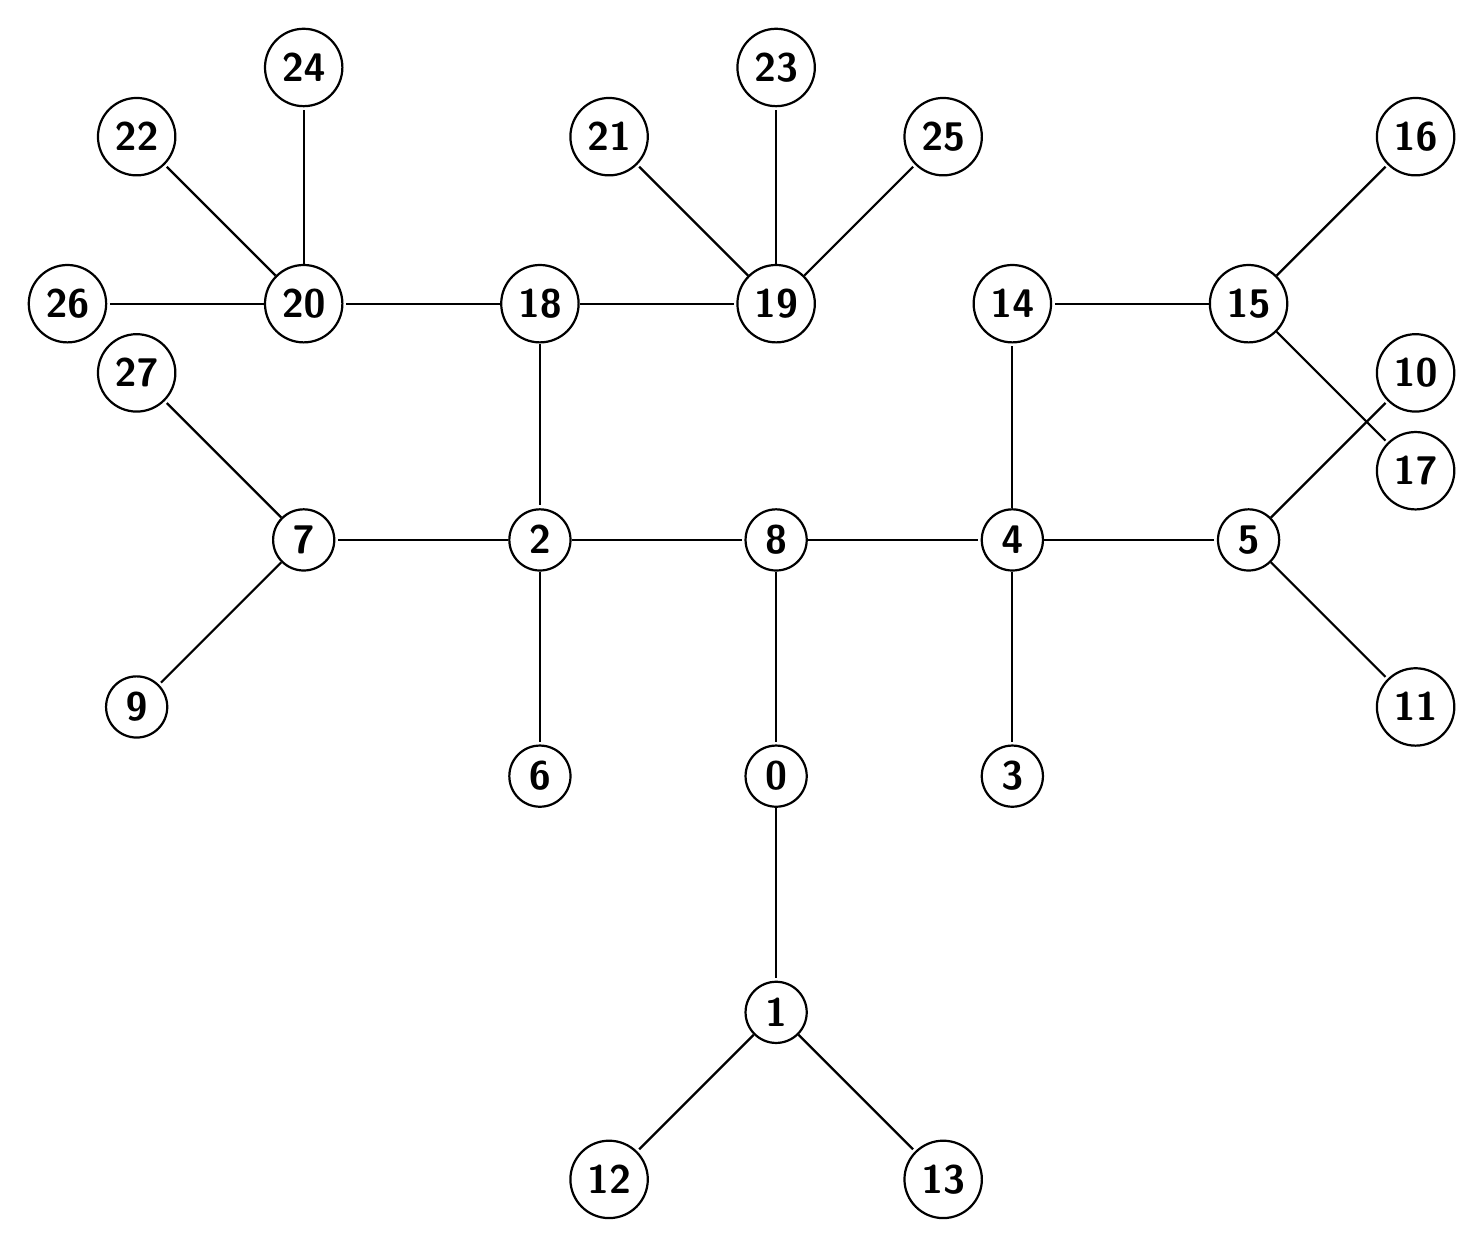
\begin{tikzpicture}[->,>=,shorten >=1pt,auto,node distance=3cm, thick,main node/.style={circle,draw,font=\sffamily\Large\bfseries}]
	
	\node[main node] (8) [yshift=.88 cm]{8};
	\node[main node] (0) [below of =8] {0};
	\node[main node] (1) [below of=0] {1};
	\node[main node] (2) [left of=8] {2};
	\node[main node] (4) [right of=8] {4};
	\node[main node] (3) [below  of=4] {3};
	\node[main node] (5) [right of=4] {5};
	\node[main node] (6) [below of=2] {6};
	\node[main node] (7) [left of=2] {7};
	\node[main node] (9) [below left of=7] {9};
	\node[main node] (27) [above left of=7] {27};

	\node[main node] (10) [above right of=5] {10};
	\node[main node] (11) [below right of=5] {11};
	\node[main node] (12) [below left of=1] {12};
	\node[main node] (13) [below right of=1] {13};
	\node[main node] (14) [above of=4] {14};
	\node[main node] (15) [right of=14] {15};
	\node[main node] (16) [above right of=15] {16};
	\node[main node] (17) [below right of=15] {17};
	
	\node[main node] (18) [above of=2] {18};
	\node[main node] (19) [right of=18] {19};
	\node[main node] (20) [left of=18] {20};
	\node[main node] (21) [above left of=19] {21};
	\node[main node] (22) [above left of=20] {22};
	\node[main node] (23) [above of=19] {23};
	\node[main node] (24) [above of=20] {24};
	\node[main node] (25) [above right of=19] {25};
	\node[main node] (26) [left of=20] {26};
 	%\coordinate (8) at ($(1)!0.5!(3)$) {8};

	\path[every node/.style={font=\sffamily\small}]
		(0) 
		edge node [] {} (1)

		(1)
		edge node [left] {} (12)
		edge node [left] {} (13)
		
		(2) 
		edge node [right] {} (8)
		edge node {} (7)
		edge node [below] {} (6)
		
		(3) 

		
		(4) 
		edge node [left] {} (3)
		edge node [right]   {} (5)
		edge node [above]	{} (14)
		
		(5)
		edge node [right] {} (10)
		edge node [right] {} (11)
		
		(7)
		edge node [left] {}(9)
		edge node [left] {}(27)
		
		(8) 
		edge node [right]	{} (4)
		edge node [below] {} (0)
		
		(15)
		edge node [right]	{} (16)
		edge node [right]	{} (17)
		edge node [left]	{} (14)
		
		(18)
		edge node [below]	{} (2)
		edge node [right]	{} (19)
		edge node [left]	{} (20)
		
		(19)
		edge node [left]	{} (21)
		edge node [above]	{} (23)
		edge node [right]	{} (25)
		
		(20)
		edge node [above left]	{} (22)
		edge node [above]	{} (24)
		edge node [left]	{} (26)
		;
		      
		

	\end{tikzpicture}
	
	
	%/*%
	%  edge [loop right] node {0.6} (4)
	%edge [bend right] node[right] {0.2} (1);
	%*/
\end{center}

% Albero B
\paragraph{\newline Grafo Generato Ciclico \newline}
\begin{center}
	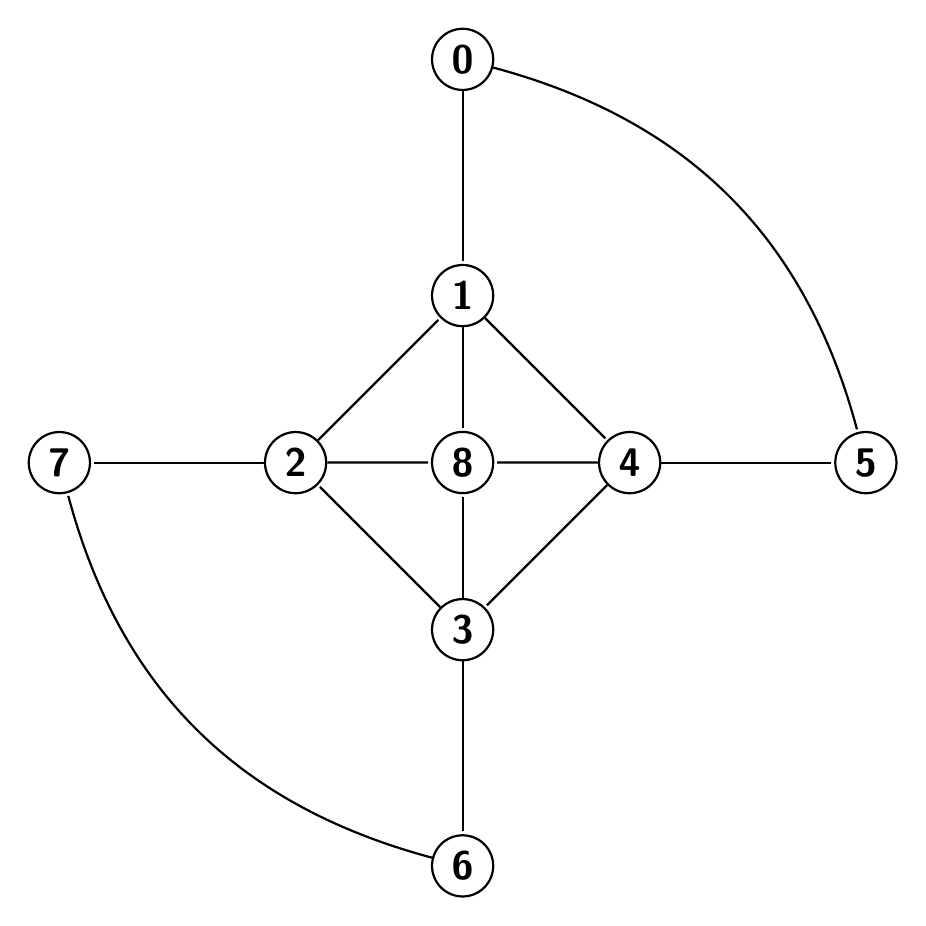
\begin{tikzpicture}[->,>=,shorten >=1pt,auto,node distance=3cm, thick,main node/.style={circle,draw,font=\sffamily\Large\bfseries}]
	
	\node[main node] (0) {0};
	\node[main node] (1) [below of=0] {1};
	\node[main node] (2) [below left of=1] {2};
	\node[main node] (3) [below right of=2] {3};
	\node[main node] (4) [below right of=1] {4};
	\node[main node] (5) [right of=4] {5};
	\node[main node] (6) [below of=3] {6};
	\node[main node] (7) [left of=2] {7};
	\node[main node] (8) [below of=1, yshift=.88 cm]{8};
 	%\coordinate (8) at ($(1)!0.5!(3)$) {8};
	
	\path[every node/.style={font=\sffamily\small}]
		(0) edge node [] {} (1)
			  edge [bend left] node[] {} (5)
			
		(1)	edge node [left] {} (4)
			 edge node [below] {} (8)
		(2) edge node [right] {} (1)
		edge node {} (8)
		edge node {} (7)
		(3) edge node [right] {} (2)
			  edge node [below] {} (6)
			  edge node [above] {} (8)
		(4) edge node [left] {} (3)
		      edge node [right] {} (5)
		      edge node [left] {} (8)
		      
		 (6) edge [bend left] node [] {} (7);
		

	\end{tikzpicture}
	
	
	%/*%
	%  edge [loop right] node {0.6} (4)
	%edge [bend right] node[right] {0.2} (1);
	%*/
\end{center}

\paragraph{Attenzione:} per ragioni di DEBUG o di TESTING fornisco di seguito l'Array ed il Dizionario dei due grafi di cui sopra per permetterne la verifica dei risultati. \newline \newline
%\emph{Grafo Aciclico: \\}
%V = [ ] \\
%A = \{\}
%\newline 
%\newline
%\emph{\\ \\ Grafo Ciclico: \\}
%V = [ ] \\
%A = \{\}

\emph{ \\Grafo Aciclico: \\ \\}
V = [ 0, 1, 2, 3, 4, 5, 6, 7, 8, 9, 10, 11, 12, 13, 14, 15, 16, 17, 18, 19, 20, 21, 22, 23, 24, 25, 26, 27 ]
\\ \\
A = \{ 0:[1, 8],  1:[0, 12, 13], 2:[7, 18, 8, 6], 3:[4], 4:[8, 14, 5, 3], 5:[4, 10, 11], 6:[2], 7:[27, 2, 9], 8:[2, 4, 0], 9:[7], 10:[5], 11:[5], 12:[1], 13:[1], 14:[4, 15], 15:[14, 16, 17], 16:[15], 17:[15], 18:[20, 19, 2], 19:[18, 21, 23, 25], 20:[26, 22, 24, 18], 21:[19], 22:[20], 23:[19], 24:[20], 25:[19], 26:[20], 27:[7]\}
\\ \\
R: (442.0, \{2\}, \{0: 144.0, 1: 102.0, 2: 442.0, 3: 0, 4: 342.0, 5: 102.0, 6: 0, 7: 102.0, 8: 436.0, 9: 0, 10: 0, 11: 0, 12: 0, 13: 0, 14: 144.0, 15: 102.0, 16: 0, 17: 0, 18: 336.0, 19: 150.0, 20: 150.0, 21: 0, 22: 0, 23: 0, 24: 0, 25: 0, 26: 0, 27: 0\})


\emph{\\ \\ Grafo Ciclico: \\ \\}
V = [0, 1, 2, 3, 4, 5, 6, 7, 8]
\\ \\
A = \{ 0:[1, 5], 1:[2, 0, 4, 8], 2:[7, 1, 8, 3], 3:[2, 8, 4, 6], 4:[8, 1, 5, 3], 5:[4, 0], 6:[7, 3], 7:[2, 6], 8:[2, 1, 4, 3] \}
\\ \\
R: (17.06666666666667, \{1\}, \{0: 1.9, 1: 17.06666666666667, 2: 17.066666666666666, 3: 17.066666666666666, 4: 17.066666666666666, 5: 1.9, 6: 1.9, 7: 1.9, 8: 4.133333333333334\})
\\
\noindent 
\paragraph{Attenzione:}Come si può evincere dalla quantità di dati e dal Return dell'algoritmo, a grafi complessi corrispondo valori di Betweennes Centrality più complessi e più raffinati, al fine di semplificarne l'analisi è ovviamente implementabile la \emph{normalizzazione} dei dati come è già di per se fatto all'interno di librerie come la NetworkX ( Python ).


\newpage

\section{Inizializzazione}
$\mathbf{Tempo: O(n)}$\\ 	\\
L'inizializzazione dell'algoritmo consta di alcuni allocamenti preventivi di spazio in memoria, procede quindi ad inizializzare da subito il dizionario "R" ponendo a zero tutti i valori ed indicizzandoli con gli ID dei nodi del grafo. Procede quindi ad iterare su ogni singolo nodo del grafo da cui si evince subito che l'algoritmo si carica di una complessità temporale $O(n)$

\section{Calcolo dei Cammini Minimi}
$\mathbf{Tempo: O(m)}$\\ 	\\
Esegue una visita del grafo a partire dall'attuale nodo esaminato ( praticamente una BFS nel caso di grafi non pesati ), la particolarità è il suo tempo di esecuzione che, secondo il Corollario 4 del Paper di Brandes, sia pari ad $O(m)$
Durante questa visita vengono computati l'insieme \emph{pred(s,v)} dei predecessori che giacciono sui cammini mini ed il numero di quest'ultimi tra $s$ e $v$ ( $\delta_{sv}$ )

\section{Calcolo e somma delle Dipendenze}
$\mathbf{Tempo: O(m)}$\\ 	\\
Terminato il calcolo dei cammini minimi, del loro numero e la popolazione dell'insieme \emph{pred(s,v)} dei predecessori,  l'algoritmo itera su tutti i nodi presenti nella pila salvati durante il calcolo dei cammini minimi e ne computa le rispettive dipendenze rispetto al nodo in esame. Nel corso del calcolo viene costantemente aggiornato l'indice di \emph{Betweennes Centrality} come valore all'interno del dizionario dei risultati la cui corrispondente chiave è rappresentata dall'ID del nodo esaminato.

\section{Restituzione del risultato}
Al termine del ciclo più esterno avviato con l'inizializzazione dell'algoritmo stesso viene restituito il dizionario contenente tutti gli indici di \emph{Betweennes Centrality} indicizzati proprio dagli ID dei nodi esaminati.

